\documentclass[tikz,border=15pt]{standalone}
\usepackage{tikz}
\usetikzlibrary{shapes.geometric, arrows.meta, positioning, calc}

\tikzset{
    register/.style={
        rectangle, draw=black, thick,
        minimum width=1.6cm, minimum height=1cm,
        fill=white, font=\small\ttfamily
    },
    mux/.style={
        trapezium, trapezium left angle=70, trapezium right angle=110,
        draw=black, thick,
        minimum width=1cm, minimum height=0.9cm,
        fill=white, font=\small
    },
    alu/.style={
        rectangle, draw=black, thick,
        minimum width=1.3cm, minimum height=1.1cm,
        fill=white, font=\small
    },
    wire/.style={draw=black, thick, -Stealth},
    bus/.style={draw=black, line width=1.8pt, -Stealth},
    controlwire/.style={draw=black!60, dashed, -Stealth},
    buswidth/.style={font=\scriptsize, fill=white, inner sep=2pt},
    logic/.style={
        rectangle, draw=black, thick, rounded corners=3pt,
        minimum width=1cm, minimum height=0.9cm,
        fill=gray!10, font=\small
    },
    sbox/.style={
        rectangle, draw=black, thick,
        minimum width=0.7cm, minimum height=0.7cm,
        fill=gray!20, font=\small
    }
}

\begin{document}
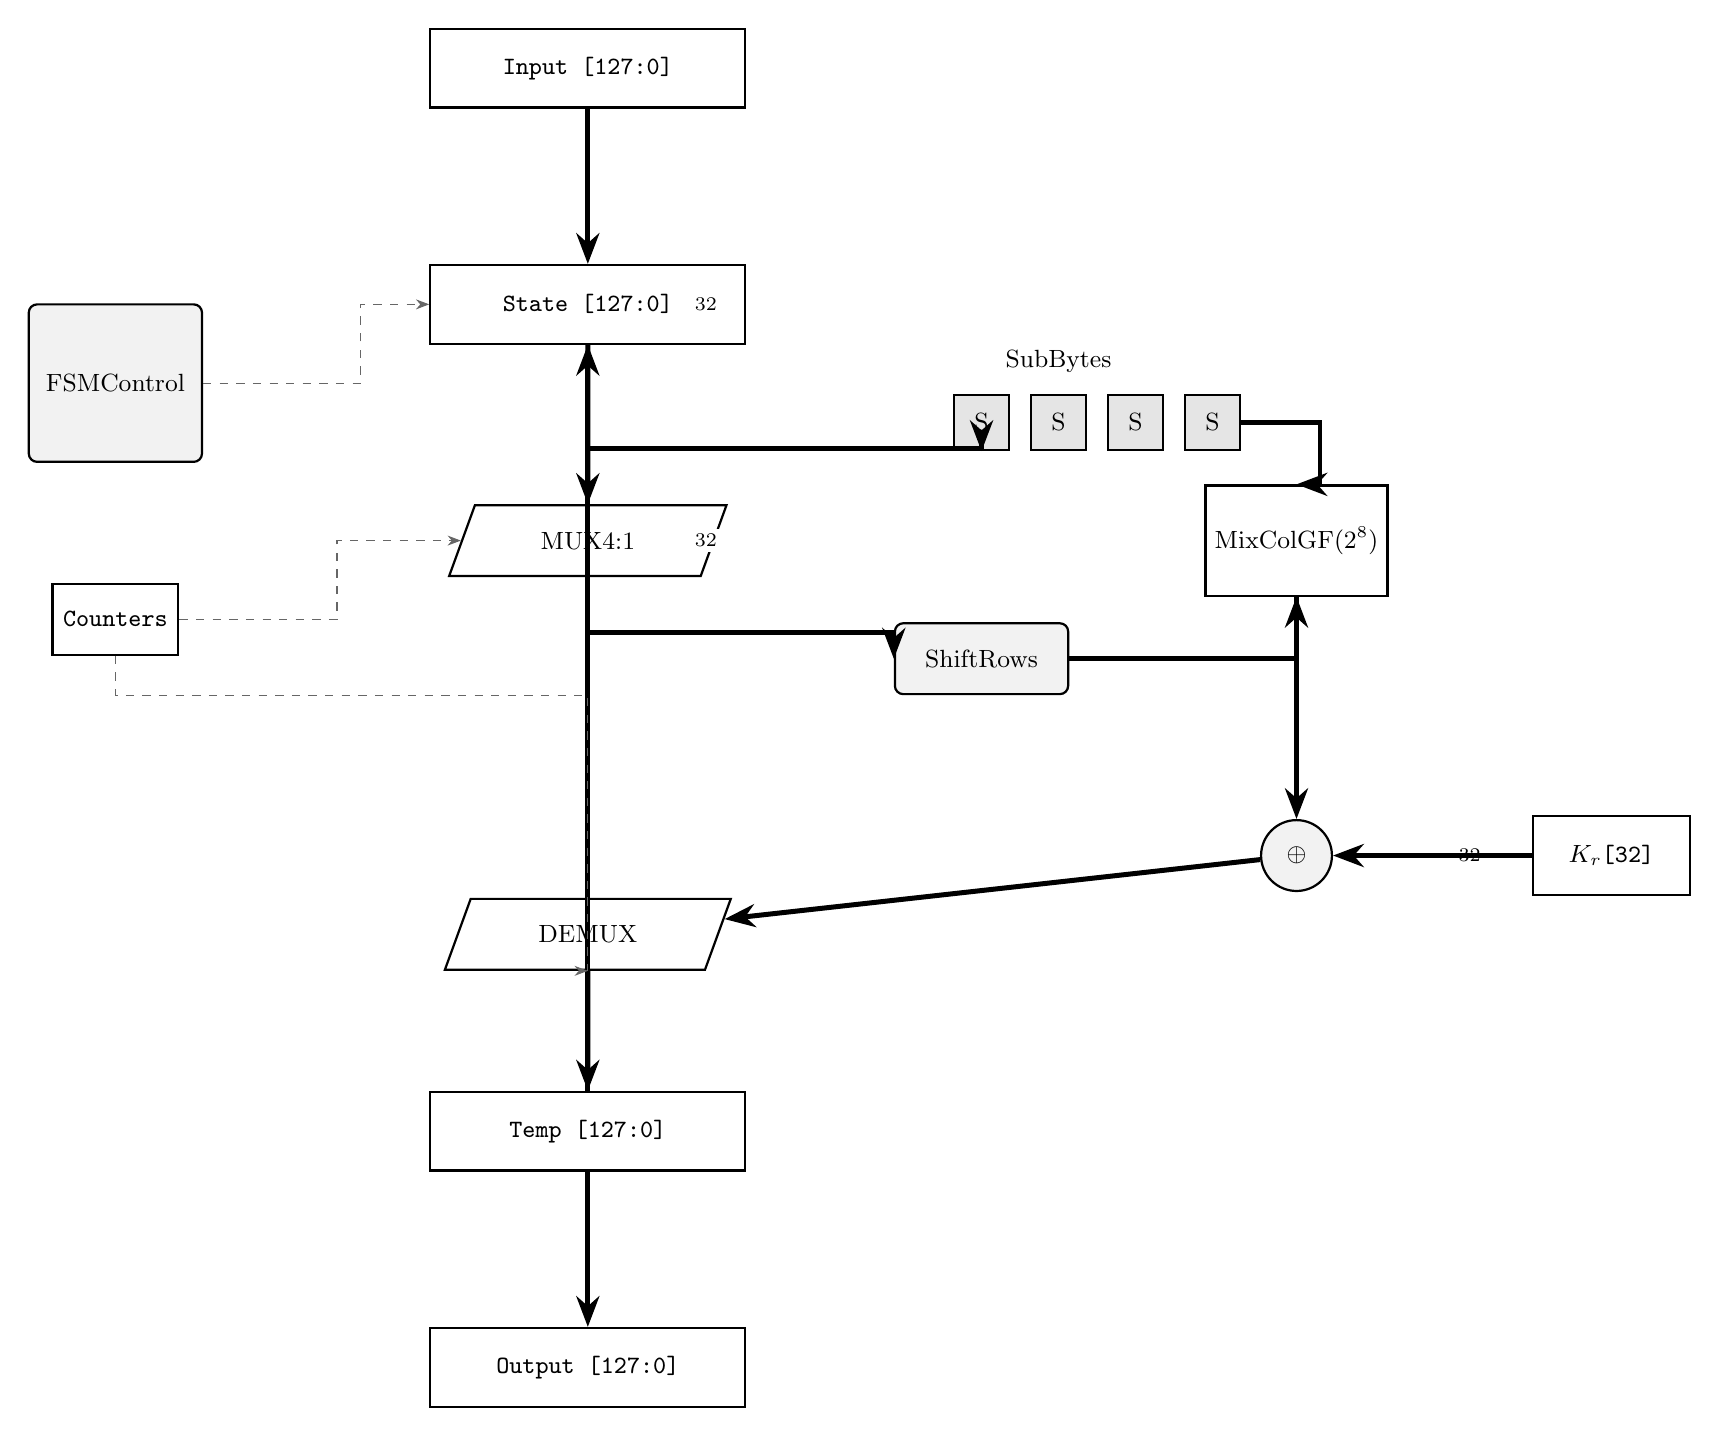
\begin{tikzpicture}

% Column 1: Control
\node[logic, minimum width=2.2cm, minimum height=2cm] (fsm) at (0,6) {FSM\\Control};
\node[register, minimum width=1.6cm, minimum height=0.9cm] (counters) at (0,3) {Counters};

% Column 2: Main datapath
\node[register, minimum width=4cm] (input_reg) at (6,10) {Input [127:0]};
\node[register, minimum width=4cm] (state_reg) at (6,7) {State [127:0]};
\node[mux, minimum width=1.2cm] (col_mux) at (6,4) {MUX\\4:1};
\node[mux, shape border rotate=180, minimum width=1.2cm] (demux) at (6,-1) {DEMUX};
\node[register, minimum width=4cm] (temp_reg) at (6,-3.5) {Temp [127:0]};
\node[register, minimum width=4cm] (output_reg) at (6,-6.5) {Output [127:0]};

% Column 3: Processing units
\node[sbox] (sbox0) at (11,5.5) {S};
\node[sbox, right=0.25cm of sbox0] (sbox1) {S};
\node[sbox, right=0.25cm of sbox1] (sbox2) {S};
\node[sbox, right=0.25cm of sbox2] (sbox3) {S};
\node[font=\small, above=0.15cm of sbox1.north] {SubBytes};

\node[logic, minimum width=2.2cm] (shift) at (11,2.5) {ShiftRows};

% Column 4: MixColumns and XOR
\node[alu, minimum width=2cm, minimum height=1.4cm] (mixcol) at (15,4) {MixCol\\GF($2^8$)};
\node[logic, circle, minimum size=0.9cm] (xor) at (15,0) {$\oplus$};

% Column 5: Round key
\node[register, minimum width=2cm] (key_word) at (19,0) {$K_r$[32]};

% Buswidth labels
\node[buswidth] at (7.5,7) {32};
\node[buswidth] at (7.5,4) {32};
\node[buswidth] at (17.2,0) {32};

% Data connections
\draw[bus] (input_reg) -- (state_reg);
\draw[bus] (state_reg) -- (col_mux);
\draw[bus] (col_mux.north) -- ++(0,0.7) -| (sbox0.south);
\draw[bus] (sbox3.east) -- ++(1,0) |- (mixcol.north);
\draw[bus] (col_mux.south) -- ++(0,-0.7) -| (shift.west);
\draw[bus] (shift.east) -| (mixcol.south);
\draw[bus] (mixcol) -- (xor);
\draw[bus] (xor) -- (demux);
\draw[bus] (demux) -- (temp_reg);
\draw[bus] (temp_reg) -- (state_reg);
\draw[bus] (temp_reg) -- (output_reg);
\draw[bus] (key_word) -- (xor);

% Control signals
\draw[controlwire] (fsm.east) -- ++(2,0) |- (state_reg.west);
\draw[controlwire] (counters.east) -- ++(2,0) |- (col_mux.west);
\draw[controlwire] (counters.south) -- ++(0,-0.5) -- ++(6,0) |- (demux.south);

\end{tikzpicture}
\end{document}
